\part{Optimisation Process}
\frame{\partpage}

\begin{frame}{Understand}
	\begin{itemize}
		\item A few things to note when optimising
		\begin{itemize}
			\item Limitations of the target hardware
			\item Understand how the CPU/GPU works
			\item Understand how your chosen engine works
			\item Understand how your chosen language compiles
		\end{itemize}
		\item For these workshops we are going to focus on a couple of these
	\end{itemize}
\end{frame}

\begin{frame}{Optimisation Process}
	\begin{itemize}
		\item Think of the quote in the intro, you should not worry about premature optimisation
		\item Get your core systems working and start optimising
		\item Make it a habit and part of your development process, not just when performance becomes a problem
		\item Every programmer in the team should optimise
	\end{itemize}
\end{frame}

\begin{frame}{Optimisation Cycle 1}
	\begin{center}
		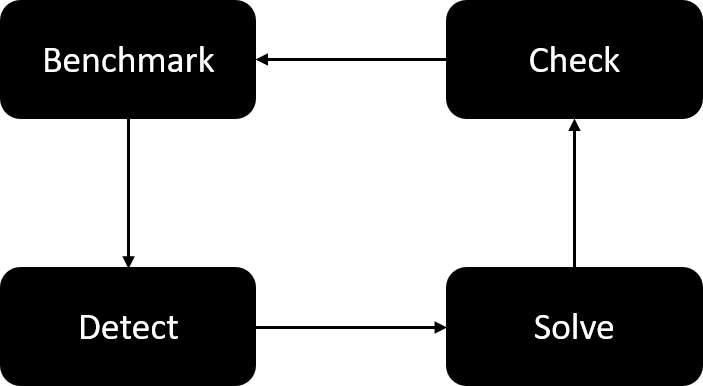
\includegraphics[width=\textwidth,height=\textheight,keepaspectratio]{optimisation_cycle}
	\end{center}
\end{frame}

\begin{frame}{Optimisation Cycle 2}
	\begin{itemize}
		\item If you look at the previous slide, these steps feel like an \textbf{experiment}
		\item We just don't try to optimise \textbf{without} data
		\item We always \textbf{profile} and find out the bottle necks and hotspots
		\item We then make changes to our code base or content
		\item Then we return to start of the process using our benchmark as a comparison
	\end{itemize}
\end{frame}


